\documentclass[12pt,a4paper]{article}
\usepackage{amsmath, amssymb, geometry, booktabs, xcolor, hyperref,
            listings, pgfplots, tcolorbox, enumitem, fancyhdr, tikz, array}
\usepgfplotslibrary{fillbetween}
\geometry{margin=2.5cm}
\pgfplotsset{compat=1.18}
\tcbuselibrary{skins, breakable}

% Define custom environments
\newtcolorbox{curiositybox}[1]{colback=yellow!10, colframe=orange!80, title=#1, breakable}
\newtcolorbox{infobox}[1]{colback=blue!5, colframe=blue!60, title=#1, breakable}
\newtcolorbox{mistakebox}[1]{colback=red!5, colframe=red!60, title=#1, breakable}
\newtcolorbox{learnbox}[1]{colback=green!5, colframe=green!60, title=#1, breakable}

% Header and Footer
\pagestyle{fancy}
\fancyhf{}
\lhead{Curvature, Evolute and Involute}
\rhead{Unit 3 -- LAC}
\cfoot{\thepage}

% Document Title Setup
\title{\textbf{Curvature of Plane Curves, Evolute and Involute} \\ \large Unit 3 -- Single Variable Calculus and Series Expansions}
\author{Department of Mathematics}
\date{\today}

\begin{document}
\maketitle
\tableofcontents
\newpage

%=============================================================
\section{Real-World Engineering Hook}
%=============================================================

\begin{curiositybox}{Why Should an Engineer Care?}
\textbf{Scenario 1 -- Highway Design:} A highway engineer designs a curved road. If the radius of curvature $R$ is too small, vehicles travelling at the design speed cannot safely navigate it: the required centripetal force exceeds the available tyre friction, and accidents occur. Minimum $R$ is computed directly from the curvature formula --- this is a life-safety calculation.

\medskip
\textbf{Scenario 2 -- Beam Bending (Euler--Bernoulli):} In structural engineering the bending moment is
\[
  M = \frac{EI}{R},
\]
where $E$ is Young's modulus, $I$ is the second moment of area, and $R$ is the radius of curvature of the deflected beam. An incorrect $R$ produces wrong stress estimates and can cause catastrophic structural failure.

\medskip
\textbf{Scenario 3 -- Involute Gear Teeth:} The standard profile for spur gear teeth worldwide is the \emph{involute of a circle}. It guarantees a constant velocity ratio between meshing gears regardless of centre-distance variation. Without involute geometry, gear pairs screech, wear prematurely, and fail under load.

\medskip
\textbf{Scenario 4 -- CNC Machining and Cam Design:} Computer-controlled cutting tools follow curvature-based toolpaths. Incorrect curvature calculations lead to dimensional inaccuracies, surface finish defects, and tool breakage. Cam profiles rely on evolute geometry to control follower acceleration profiles precisely.
\end{curiositybox}

%=============================================================
\section{Why This Topic Exists}
%=============================================================

\begin{center}
\begin{tabular}{@{}p{4.5cm} p{9cm}@{}}
\toprule
\textbf{Theoretical Concept} & \textbf{Engineering Application / Consequence of Misunderstanding} \\
\midrule
Curvature $\kappa$ & Quantifies sharpness of turns; misapplied in highway design leads to unsafe curves and accidents \\[4pt]
Radius of Curvature (Cartesian, Parametric, Polar) & Direct input to beam bending $M=EI/R$; polar form essential for polar-defined mechanisms such as spirals and cardioids \\[4pt]
Centre of Curvature & Locates osculating circle centre; critical for cam and gear tooth profile design \\[4pt]
Circle of Curvature (Osculating Circle) & Defines local second-order geometry; used in CNC toolpath generation and optical surface grinding \\[4pt]
Evolute of a Curve & Envelope of normals; used in optics (caustic curves), civil engineering (transition curves), and cam design \\[4pt]
Involute of a Curve & Standard gear tooth profile (involute of a circle); used in timing belts, mechanical transmissions, and pump impellers \\
\bottomrule
\end{tabular}
\end{center}

\begin{learnbox}{Core Learning Objective}
By the end of this unit the student will be able to compute curvature $\kappa$ and radius of curvature $R$ in Cartesian, parametric, and polar forms; find the centre and osculating circle at any smooth point; derive the evolute of a given plane curve; and derive the involute of a circle for gear tooth applications.
\end{learnbox}

%=============================================================
\section{Intuition First and Mathematical Definitions}
%=============================================================

% ---- Sub-topic 1 ----
\subsection{Curvature of Plane Curves}

Imagine driving along a curved road. On a motorway straight, you barely turn the steering wheel --- $\kappa \approx 0$. On a hairpin mountain bend, you turn it sharply --- $\kappa$ is large. Curvature $\kappa$ measures the \emph{rate at which the tangent direction rotates} per unit arc length. A perfect circle of radius $r$ has constant curvature $\kappa = 1/r$ everywhere.

\begin{infobox}{Curvature of Plane Curves --- Definitions and Formulas}
\textbf{Intrinsic Definition.}
\[
  \kappa = \left|\frac{d\phi}{ds}\right|,
\]
where $\phi$ is the inclination of the tangent and $s$ is arc length. Units: radians per metre (or per unit length).

\medskip
\textbf{Cartesian Form} $y = f(x)$:
\[
  \kappa = \frac{|y''|}{\bigl(1 + y'^{2}\bigr)^{3/2}}, \qquad y' = \frac{dy}{dx},\quad y'' = \frac{d^{2}y}{dx^{2}}.
\]

\textbf{Parametric Form} $x = x(t),\; y = y(t)$:
\[
  \kappa = \frac{|\dot{x}\ddot{y} - \ddot{x}\dot{y}|}{\bigl(\dot{x}^{2}+\dot{y}^{2}\bigr)^{3/2}}, \qquad \dot{x} = \frac{dx}{dt},\quad \ddot{x} = \frac{d^{2}x}{dt^{2}},\; \text{etc.}
\]

\textbf{Key Special Cases:}
\begin{itemize}[nosep]
  \item Straight line: $\kappa = 0$ (tangent direction never changes).
  \item Circle of radius $r$: $\kappa = \dfrac{1}{r}$ (constant).
  \item High $\kappa$ means a sharp bend; low $\kappa$ means nearly straight.
\end{itemize}
\end{infobox}

\textbf{Worked Example 1.1 --- Curvature of $y = x^2$ at $(0,0)$ and $(1,1)$.}

\medskip
\textit{Setup:} $y = x^2$, so $y' = 2x$ and $y'' = 2$.

\medskip
\textit{At $(0, 0)$} (i.e.\ $x = 0$):
\[
  \kappa(0) = \frac{|y''(0)|}{\bigl(1 + [y'(0)]^{2}\bigr)^{3/2}} = \frac{|2|}{(1 + 0^{2})^{3/2}} = \frac{2}{1} = 2.
\]

\textit{At $(1, 1)$} (i.e.\ $x = 1$):
\[
  \kappa(1) = \frac{|2|}{\bigl(1 + (2\cdot 1)^{2}\bigr)^{3/2}} = \frac{2}{(1 + 4)^{3/2}} = \frac{2}{5^{3/2}} = \frac{2}{5\sqrt{5}} = \frac{2\sqrt{5}}{25} \approx 0.179.
\]

\textit{Interpretation:} The parabola is most sharply curved at its vertex $(0,0)$ and flattens out as $x$ increases.

% ---- Sub-topic 2 ----
\subsection{Radius of Curvature (Cartesian, Parametric, and Polar Forms)}

Every smooth curve can locally be approximated by a circle. The radius of that circle is $R = 1/\kappa$. For a motorway curve the designer specifies a minimum $R$ (say 500 m for a 100 km/h road); the parabolic or circular alignment must satisfy this. When the curve is given in polar coordinates --- a cardioid, lemniscate, or Archimedean spiral --- the polar formula for $R$ must be used directly.

\begin{infobox}{Radius of Curvature --- All Three Coordinate Forms}
\textbf{Definition:} $R = \dfrac{1}{\kappa}$.

\medskip
\textbf{Cartesian} $y = f(x)$:
\[
  R = \frac{\bigl(1 + y'^{2}\bigr)^{3/2}}{|y''|}.
\]

\textbf{Parametric} $x=x(t), y=y(t)$:
\[
  R = \frac{\bigl(\dot{x}^{2}+\dot{y}^{2}\bigr)^{3/2}}{|\dot{x}\ddot{y} - \ddot{x}\dot{y}|}.
\]

\textbf{Polar} $r = f(\theta)$, with $r' = dr/d\theta$ and $r'' = d^{2}r/d\theta^{2}$:
\[
  R = \frac{\bigl(r^{2}+r'^{2}\bigr)^{3/2}}{\bigl|r^{2}+2r'^{2}-r\,r''\bigr|}.
\]

\textbf{Special cases:} Straight line $\Rightarrow R = \infty$; circle of radius $a \Rightarrow R = a$.
\end{infobox}

\textbf{Worked Example 2.1 --- Radius of Curvature of $y = x^2$ at $(1,1)$ (Cartesian).}

$y' = 2x$, $y'' = 2$. At $x = 1$: $y'(1) = 2$, $y''(1) = 2$.
\[
  R = \frac{(1 + 2^{2})^{3/2}}{|2|} = \frac{(5)^{3/2}}{2} = \frac{5\sqrt{5}}{2} \approx \frac{11.18}{2} \approx 5.59.
\]

\medskip
\textbf{Worked Example 2.2 --- Polar Form: Cardioid $r = a(1+\cos\theta)$ at $\theta = \pi/2$.}

\textit{Compute derivatives with respect to $\theta$:}
\[
  r = a(1+\cos\theta), \qquad r' = -a\sin\theta, \qquad r'' = -a\cos\theta.
\]

\textit{At $\theta = \pi/2$:}
\[
  r = a(1+0) = a,\quad r' = -a(1) = -a,\quad r'' = -a(0) = 0.
\]

\textit{Numerator:}
\[
  \bigl(r^{2}+r'^{2}\bigr)^{3/2} = \bigl(a^{2}+a^{2}\bigr)^{3/2} = (2a^{2})^{3/2} = 2\sqrt{2}\,a^{3}.
\]

\textit{Denominator:}
\[
  \bigl|r^{2}+2r'^{2}-r\,r''\bigr| = \bigl|a^{2}+2a^{2}-a\cdot 0\bigr| = |3a^{2}| = 3a^{2}.
\]

\[
  \boxed{R\!\left(\theta=\tfrac{\pi}{2}\right) = \frac{2\sqrt{2}\,a^{3}}{3a^{2}} = \frac{2\sqrt{2}\,a}{3}.}
\]

% ---- Sub-topic 3 ----
\subsection{Centre of Curvature}

The tangent line at a curve point $P$ tells us the direction of the curve. The \emph{principal normal} is perpendicular to the tangent and points toward the centre of curvature $C$. The centre lies at distance $R$ from $P$ along this normal. Knowing $C$ is essential for gear tooth and cam profile design: the cutting tool must be positioned at $C$ to generate the correct surface.

\begin{infobox}{Centre of Curvature --- Formulas and Geometry}
For a curve $y = f(x)$, at the point $(x, y)$, the \textbf{centre of curvature} $(\alpha, \beta)$ is:
\[
  \alpha = x - \frac{y'(1+y'^{2})}{y''}, \qquad \beta = y + \frac{1+y'^{2}}{y''}.
\]

\textbf{Geometric Properties:}
\begin{itemize}[nosep]
  \item $(\alpha, \beta)$ lies on the principal normal to the curve at $(x, y)$.
  \item Distance from $(x, y)$ to $(\alpha, \beta)$ equals $R = \dfrac{(1+y'^{2})^{3/2}}{|y''|}$.
  \item As $(x, y)$ moves along the curve, $(\alpha, \beta)$ traces the \emph{evolute}.
  \item The centre of curvature is the centre of the osculating (best-fitting) circle.
\end{itemize}
\end{infobox}

\textbf{Worked Example 3.1 --- Centre of Curvature of $y = x^2$ at $(1,1)$.}

$y' = 2x$, $y'' = 2$. At $(1,1)$: $y'(1) = 2$, $y''(1) = 2$.
\[
  \alpha = 1 - \frac{2(1+4)}{2} = 1 - \frac{10}{2} = 1 - 5 = -4.
\]
\[
  \beta = 1 + \frac{1+4}{2} = 1 + \frac{5}{2} = 1 + 2.5 = 3.5.
\]

\textit{Centre of curvature at $(1,1)$ for $y=x^{2}$ is $\boldsymbol{(\alpha,\beta) = (-4,\; 3.5)}$.}

\textit{Verification:} Distance $= \sqrt{(1-(-4))^{2}+(1-3.5)^{2}} = \sqrt{25+6.25} = \sqrt{31.25} = \dfrac{5\sqrt{5}}{2} = R$. \checkmark

% ---- Sub-topic 4 ----
\subsection{Circle of Curvature (Osculating Circle)}

Among all circles tangent to a curve at point $P$, the \emph{osculating circle} is the unique one that also matches the curvature of the curve at $P$. It is the ``best'' local circular approximation in the sense that it agrees with the curve to second order: same position, same tangent, same curvature. CNC controllers use the osculating circle to compute the offset toolpath for machining curved surfaces.

\begin{infobox}{Circle of Curvature (Osculating Circle) --- Definition and Equation}
\textbf{Definition:} The osculating circle at a point $P = (x_0, y_0)$ on a smooth curve is the unique circle that:
\begin{enumerate}[nosep]
  \item Passes through $P$.
  \item Has the same tangent as the curve at $P$.
  \item Has the same curvature $\kappa$ (equivalently, radius $R = 1/\kappa$) as the curve at $P$.
\end{enumerate}

\textbf{Equation of the Osculating Circle:}
\[
  (x - \alpha)^{2} + (y - \beta)^{2} = R^{2},
\]
where $(\alpha, \beta)$ is the centre of curvature and $R$ is the radius of curvature at $P$.

\textbf{Second-Order Contact:} The osculating circle agrees with the curve up to and including the second derivative at $P$. Any other tangent circle agrees only to first order (same tangent) but not to second order (different curvature).

\textbf{Uniqueness:} At each smooth point with $\kappa \neq 0$, the osculating circle is unique.
\end{infobox}

\textbf{Worked Example 4.1 --- Osculating Circle for $y = x^3$ at $(1, 1)$.}

\textit{Derivatives:} $y' = 3x^{2}$, $y'' = 6x$.

\textit{At $(1,1)$:} $y'(1) = 3$, $y''(1) = 6$.

\textit{Radius of curvature:}
\[
  R = \frac{(1+9)^{3/2}}{6} = \frac{10^{3/2}}{6} = \frac{10\sqrt{10}}{6} = \frac{5\sqrt{10}}{3} \approx \frac{15.81}{3} \approx 5.27.
\]

\textit{Centre of curvature:}
\[
  \alpha = 1 - \frac{3(1+9)}{6} = 1 - \frac{30}{6} = 1 - 5 = -4.
\]
\[
  \beta = 1 + \frac{1+9}{6} = 1 + \frac{10}{6} = 1 + \frac{5}{3} = \frac{8}{3} \approx 2.667.
\]

\textit{Equation of the osculating circle:}
\[
  \boxed{(x+4)^{2} + \left(y - \frac{8}{3}\right)^{2} = \frac{250}{9}.}
\]

\textit{Verification that $(1,1)$ lies on the circle:}
\[
  (1+4)^{2} + \left(1-\frac{8}{3}\right)^{2} = 25 + \left(-\frac{5}{3}\right)^{2} = 25 + \frac{25}{9} = \frac{225+25}{9} = \frac{250}{9} = R^{2}.\quad\checkmark
\]

% ---- Sub-topic 5 ----
\subsection{Evolute of a Curve}

As point $P$ slides along a curve $C$, the centre of curvature $(\alpha, \beta)$ traces a new curve called the \emph{evolute} of $C$. Every normal to $C$ is tangent to the evolute --- the evolute is the \emph{envelope of the family of normals}. In optics, the evolute is the caustic curve (the bright line formed when parallel rays reflect off a curved mirror). In civil engineering, transition (spiral) curves use evolute properties to ensure smooth curvature changes.

\begin{infobox}{Evolute of a Curve --- Definition and Properties}
\textbf{Definition:} The evolute of a plane curve $C$ is the locus of the centres of curvature of $C$. If $C$ is parametrised by $t$, with centre of curvature $(\alpha(t), \beta(t))$, then the evolute has parametric equations:
\[
  X = \alpha(t), \qquad Y = \beta(t),
\]
where
\[
  \alpha = x - \frac{y'(1+y'^{2})}{y''}, \qquad \beta = y + \frac{1+y'^{2}}{y''}.
\]

\textbf{Key Properties:}
\begin{itemize}[nosep]
  \item Every normal to the original curve $C$ is tangent to the evolute.
  \item Equivalently, the evolute is the \emph{envelope of the normals} to $C$.
  \item If $C$ is rectified (unrolled), the evolute is the base curve from which $C$ is unwound.
  \item A curve and its evolute are related: the evolute of the involute of a curve is the original curve.
\end{itemize}
\end{infobox}

\textbf{Worked Example 5.1 --- Evolute of the Parabola $y = x^2$.}

\textit{Parametrize by $x = t$:} $y = t^{2}$, $y' = 2t$, $y'' = 2$.

\textit{Centre of curvature as a function of $t$:}
\[
  \alpha = t - \frac{2t(1+4t^{2})}{2} = t - t(1+4t^{2}) = t - t - 4t^{3} = -4t^{3}.
\]
\[
  \beta = t^{2} + \frac{1+4t^{2}}{2} = t^{2} + \frac{1}{2} + 2t^{2} = 3t^{2} + \frac{1}{2}.
\]

\textit{Eliminate the parameter $t$:} From $\alpha = -4t^{3}$ we get $t^{3} = -\alpha/4$, so $t = (-\alpha/4)^{1/3}$.

From $\beta = 3t^{2} + 1/2$ we get $t^{2} = (\beta - 1/2)/3$.

Cubing the second relation: $t^{6} = [(\beta-1/2)/3]^{3}$.

From the first: $t^{6} = (t^{3})^{2} = (\alpha/4)^{2} = \alpha^{2}/16$.

Equating:
\[
  \frac{\alpha^{2}}{16} = \frac{(\beta - 1/2)^{3}}{27}.
\]

Substituting $(X, Y)$ for $(\alpha, \beta)$ and multiplying out:
\[
  27 X^{2} = 16\!\left(Y - \tfrac{1}{2}\right)^{3}.
\]

This is the semicubical parabola (the evolute of $y = x^{2}$).

\textit{Geometric check:} The normal to $y = x^{2}$ at $(t, t^{2})$ has slope $-1/(2t)$ and passes through $(-4t^{3},\; 3t^{2}+1/2)$, confirming the normals are tangent to this evolute. \checkmark

% ---- Sub-topic 6 ----
\subsection{Involute of a Curve}

Tie a piece of string tightly around a curved spool (the base curve $C$). Grip the free end and slowly unwind the string, keeping it taut. The path traced by the free end is the \emph{involute} of $C$. Every curve has a one-parameter family of involutes (corresponding to different initial string lengths), and all of them are parallel curves of one another. The most important engineering application is the involute of a circle, which is the universal standard for gear tooth profiles.

\begin{infobox}{Involute of a Curve --- Definition and Parametric Equations}
\textbf{String-Unwinding Definition:} The involute of curve $C$ is the curve traced by the end of a taut string as it is unwound from $C$.

\textbf{Parametric Form (arc-length parametrization):}
If $C$ is given by $(x(s), y(s))$ parametrised by arc length $s$, with unit tangent $(\cos\psi(s), \sin\psi(s))$, then the involute starting at $s = s_0$ is:
\[
  X(s) = x(s) - (s - s_0)\cos\psi(s), \qquad Y(s) = y(s) - (s-s_0)\sin\psi(s).
\]

\textbf{Involute of a Circle of Radius $a$:}
Parametrize the circle as $x = a\cos\theta$, $y = a\sin\theta$. The arc length from $\theta=0$ is $s = a\theta$. The unit tangent angle is $\psi = \theta + \pi/2$. Setting $s_0 = 0$:
\[
  X(\theta) = a\cos\theta + a\theta\sin\theta = a(\cos\theta + \theta\sin\theta),
\]
\[
  Y(\theta) = a\sin\theta - a\theta\cos\theta = a(\sin\theta - \theta\cos\theta).
\]

\textbf{Key Properties:}
\begin{itemize}[nosep]
  \item The tangent to the involute at every point is perpendicular to the corresponding tangent of $C$ (i.e.\ normal to $C$).
  \item All involutes of a given curve are \emph{parallel curves} (constant normal offset from each other).
  \item The evolute of any involute of $C$ is $C$ itself: evolute and involute are inverse operations.
  \item Engineering relevance: the involute circle profile ensures a constant velocity ratio in a spur gear pair regardless of small variations in centre distance.
\end{itemize}
\end{infobox}

\textbf{Worked Example 6.1 --- Involute of a Circle of Radius $a$.}

\textit{Base curve:} Circle $x = a\cos\theta$, $y = a\sin\theta$.

\textit{Arc length from $\theta = 0$:} $s(\theta) = a\theta$ (since $ds/d\theta = a$).

\textit{Unit tangent at $\theta$:} $\left(\dfrac{dx/d\theta}{a}, \dfrac{dy/d\theta}{a}\right) = (-\sin\theta,\; \cos\theta)$.

\textit{Involute (starting from $\theta=0$, so $s_0 = 0$):}

The string has length $s - s_0 = a\theta$. The end of the string moves in the direction \emph{opposite} to the tangent (unwinding direction):
\[
  X = a\cos\theta - a\theta(-\sin\theta) = a\cos\theta + a\theta\sin\theta = a(\cos\theta + \theta\sin\theta),
\]
\[
  Y = a\sin\theta - a\theta(\cos\theta) = a(\sin\theta - \theta\cos\theta).
\]

\textit{Engineering note (gear with $a = 2$ cm):} At $\theta = \pi/4 \approx 0.785$ rad:
\[
  X = 2(\cos 45^{\circ} + 0.785\sin 45^{\circ}) = 2\bigl(0.7071 + 0.785\times 0.7071\bigr) = 2(0.7071 + 0.555) = 2(1.262) = 2.524\;\text{cm},
\]
\[
  Y = 2(\sin 45^{\circ} - 0.785\cos 45^{\circ}) = 2(0.7071 - 0.555) = 2(0.152) = 0.304\;\text{cm}.
\]

As a gear rotates, the contact point between two involute teeth moves along the \emph{line of action}, ensuring a constant velocity ratio regardless of small manufacturing errors in centre distance.

%=============================================================
\section{Visual Artifacts and Geometric Interpretation}
%=============================================================

\textbf{Figure 4.1 --- Parabola $y = x^{2}$ and its Osculating Circle at $(1,1)$.}

\begin{center}
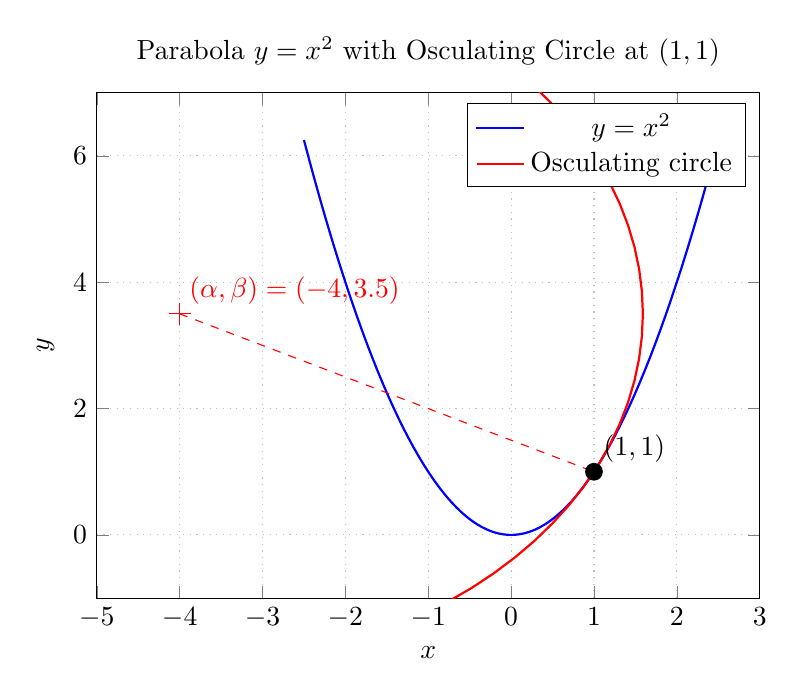
\begin{tikzpicture}
\begin{axis}[
  width=10cm, height=8cm,
  xlabel={$x$}, ylabel={$y$},
  xmin=-5, xmax=3, ymin=-1, ymax=7,
  grid=major, grid style={dotted},
  title={Parabola $y=x^2$ with Osculating Circle at $(1,1)$}
]
% Parabola
\addplot[blue, thick, domain=-2.5:2.5, samples=80] {x^2};
\addlegendentry{$y=x^2$}
% Osculating circle at (1,1): centre (-4, 3.5), radius = 5*sqrt(5)/2
% R^2 = 125/4 = 31.25
\addplot[red, thick, domain=0:360, samples=100]
  ({-4 + sqrt(31.25)*cos(x)}, {3.5 + sqrt(31.25)*sin(x)});
\addlegendentry{Osculating circle}
% Mark point (1,1)
\addplot[mark=*, mark size=3pt, black] coordinates {(1,1)};
\node[above right] at (axis cs:1,1) {$(1,1)$};
% Mark centre (-4, 3.5)
\addplot[mark=+, mark size=4pt, red] coordinates {(-4,3.5)};
\node[above right, red] at (axis cs:-4,3.5) {$(\alpha,\beta)=(-4,3.5)$};
% Radius line
\addplot[dashed, red] coordinates {(-4,3.5) (1,1)};
\node[midway, sloped, above, red] at (axis cs:-1.5,2.25) {$R\approx 5.59$};
\end{axis}
\end{tikzpicture}
\end{center}

\medskip
\textbf{Figure 4.2 --- Tangent, Normal, and Centre of Curvature on a Plane Curve.}

\begin{center}
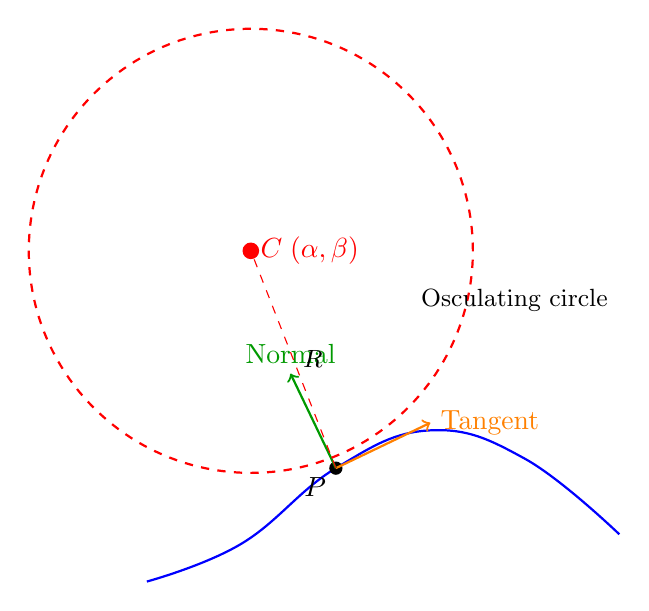
\begin{tikzpicture}[scale=1.2]
% Draw a smooth curve
\draw[blue, thick] plot[smooth, tension=0.7] coordinates
  {(0,0) (1,0.4) (2,1.2) (3,1.6) (4,1.3) (5,0.5)};
% Point P at (2,1.2)
\fill[black] (2,1.2) circle (2pt) node[below left] {$P$};
% Tangent direction (approximate)
\draw[->, thick, orange] (2,1.2) -- (3.0,1.68) node[right] {Tangent};
% Normal direction (perpendicular to tangent)
\draw[->, thick, green!60!black] (2,1.2) -- (1.52,2.2) node[above] {Normal};
% Centre of curvature C
\fill[red] (1.1,3.5) circle (2.5pt) node[right] {$C\;(\alpha,\beta)$};
% Dashed line from P to C
\draw[dashed, red] (2,1.2) -- (1.1,3.5);
\node[right] at (1.55,2.35) {\small $R$};
% Osculating circle (approximate)
\draw[red, dashed, thick] (1.1,3.5) circle (2.35cm);
\node[below right] at (2.8,3.2) {\small Osculating circle};
\end{tikzpicture}
\end{center}

\medskip
\textbf{Figure 4.3 --- Curvature $\kappa(x)$ of $y = \sin x$ on $[0, 2\pi]$.}

\begin{center}
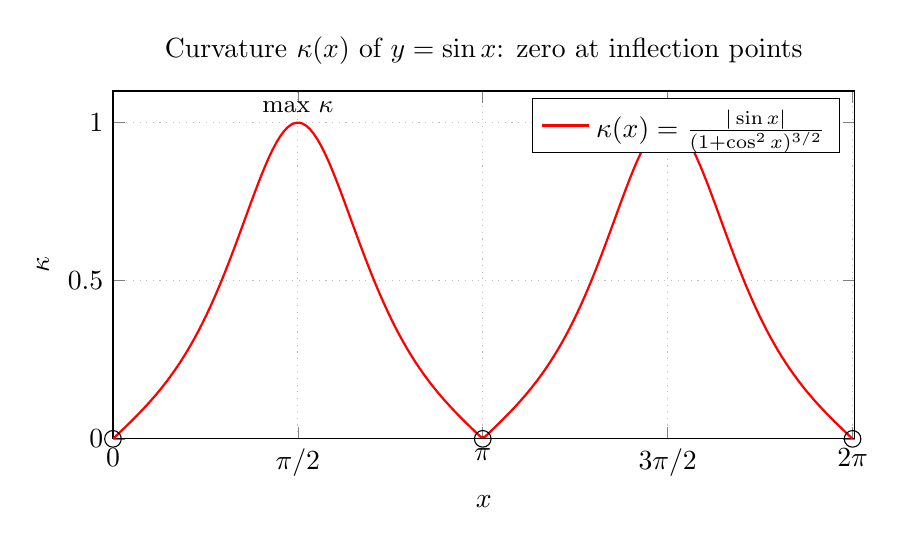
\begin{tikzpicture}
\begin{axis}[
  width=11cm, height=6cm,
  xlabel={$x$}, ylabel={$\kappa$},
  xmin=0, xmax=6.3,
  ymin=0, ymax=1.1,
  grid=major, grid style={dotted},
  xtick={0, 1.5708, 3.1416, 4.7124, 6.2832},
  xticklabels={$0$, $\pi/2$, $\pi$, $3\pi/2$, $2\pi$},
  title={Curvature $\kappa(x)$ of $y=\sin x$: zero at inflection points}
]
% kappa(x) = |cos x| / (1 + cos^2(x))^(3/2) -- but compute numerically
% y'=cos x, y''=-sin x, kappa = |sin x| / (1 + cos^2(x))^(3/2)
\addplot[red, thick, domain=0:6.2832, samples=200]
  {abs(sin(deg(x))) / (1 + (cos(deg(x)))^2)^(1.5)};
\addlegendentry{$\kappa(x) = \frac{|\sin x|}{(1+\cos^2 x)^{3/2}}$}
% Mark inflection points where kappa=0
\addplot[mark=o, mark size=3pt, black, only marks]
  coordinates {(0,0) (3.1416,0) (6.2832,0)};
\node[above] at (axis cs:1.5708,1.0) {\small max $\kappa$};
\node[above] at (axis cs:4.7124,1.0) {\small max $\kappa$};
\end{axis}
\end{tikzpicture}
\end{center}

\medskip
\textbf{Figure 4.4 --- Evolute of the Parabola $y = x^2$.}

\begin{center}
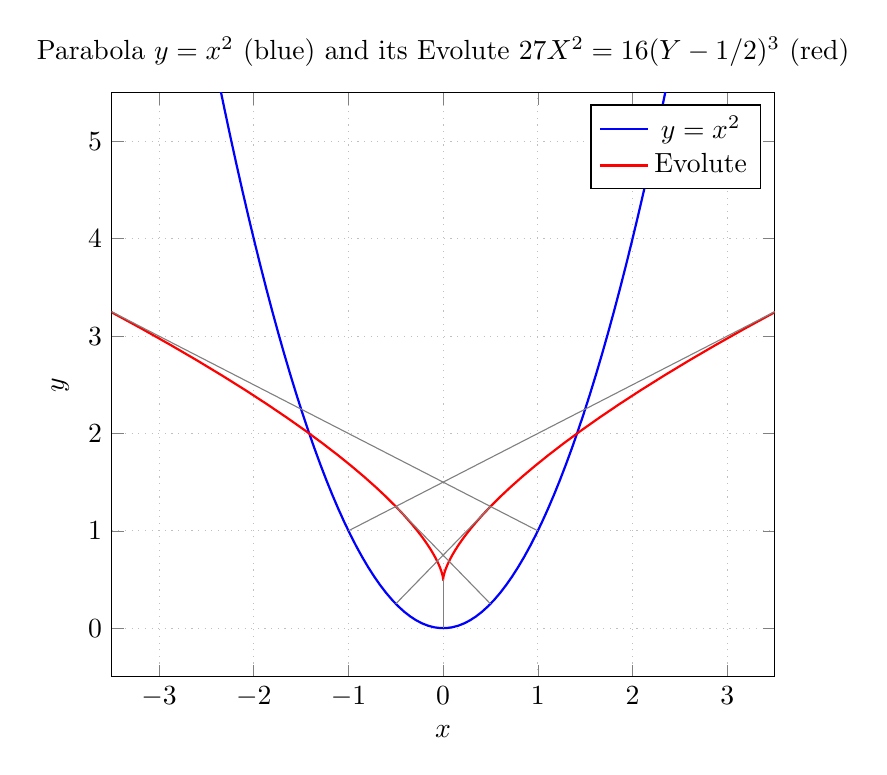
\begin{tikzpicture}
\begin{axis}[
  width=10cm, height=9cm,
  xlabel={$x$}, ylabel={$y$},
  xmin=-3.5, xmax=3.5, ymin=-0.5, ymax=5.5,
  grid=major, grid style={dotted},
  title={Parabola $y=x^2$ (blue) and its Evolute $27X^2=16(Y-1/2)^3$ (red)}
]
% Parabola y=x^2
\addplot[blue, thick, domain=-2.5:2.5, samples=80] {x^2};
\addlegendentry{$y=x^2$}
% Evolute: alpha = -4t^3, beta = 3t^2 + 1/2
\addplot[red, thick, domain=-1.2:1.2, samples=80]
  ({-4*x^3}, {3*x^2 + 0.5});
\addlegendentry{Evolute}
% Draw a few normals to the parabola at t=-1,-0.5,0,0.5,1
\addplot[gray, thin] coordinates {(-1,1) (4, 3.5)};
\addplot[gray, thin] coordinates {(-0.5,0.25) (0.5, 1.25)};
\addplot[gray, thin] coordinates {(0,0) (0, 0.5)};
\addplot[gray, thin] coordinates {(0.5,0.25) (-0.5, 1.25)};
\addplot[gray, thin] coordinates {(1,1) (-4, 3.5)};
\end{axis}
\end{tikzpicture}
\end{center}

\medskip
\textbf{Figure 4.5 --- Involute of a Circle (base circle $a = 1$).}

\begin{center}
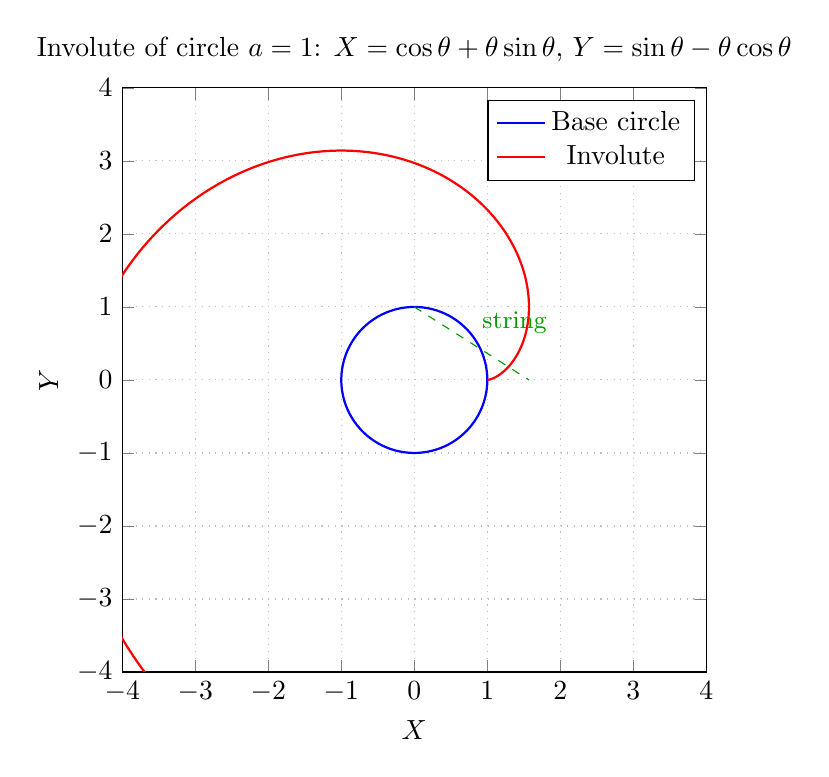
\begin{tikzpicture}
\begin{axis}[
  width=9cm, height=9cm,
  xlabel={$X$}, ylabel={$Y$},
  xmin=-4, xmax=4, ymin=-4, ymax=4,
  grid=major, grid style={dotted},
  title={Involute of circle $a=1$: $X=\cos\theta+\theta\sin\theta$, $Y=\sin\theta-\theta\cos\theta$},
  axis equal image
]
% Base circle a=1
\addplot[blue, thick, domain=0:360, samples=100]
  ({cos(x)}, {sin(x)});
\addlegendentry{Base circle}
% Involute a=1, theta from 0 to 2*pi
\addplot[red, thick, domain=0:360, samples=200]
  ({cos(x) + (x*3.14159/180)*sin(x)},
   {sin(x) - (x*3.14159/180)*cos(x)});
\addlegendentry{Involute}
% Annotate unwinding string at theta=pi/2 (90 deg)
% Point on circle: (0, 1); string end: (pi/2*1, 0) = (1.5708, 0) approx
\addplot[dashed, green!60!black]
  coordinates {(0,1) (1.5708, 0)};
\node[above right, green!60!black] at (axis cs:0.8, 0.5) {\small string};
\end{axis}
\end{tikzpicture}
\end{center}

%=============================================================
\section{Step-by-Step Algorithmic Workflow}
%=============================================================

\begin{learnbox}{Master Algorithm: Curvature, Evolute, and Involute Computations}
\textbf{Step 1 --- Curvature (Cartesian).}
Given $y = f(x)$:
\begin{enumerate}[nosep]
  \item Compute $y' = dy/dx$ and $y'' = d^{2}y/dx^{2}$.
  \item Apply $\kappa = |y''|/(1+y'^{2})^{3/2}$.
  \item Evaluate at the given point.
\end{enumerate}

\textbf{Step 2 --- Radius of Curvature (Cartesian).}
$R = (1+y'^{2})^{3/2}/|y''|$. (Reciprocal of $\kappa$.)

\textbf{Step 3 --- Radius of Curvature (Polar).}
Given $r = f(\theta)$:
\begin{enumerate}[nosep]
  \item Compute $r' = dr/d\theta$ and $r'' = d^{2}r/d\theta^{2}$.
  \item Apply $R = (r^{2}+r'^{2})^{3/2}/|r^{2}+2r'^{2}-r\,r''|$.
\end{enumerate}

\textbf{Step 4 --- Centre of Curvature.}
$\alpha = x - y'(1+y'^{2})/y''$;\quad $\beta = y + (1+y'^{2})/y''$.

\textbf{Step 5 --- Osculating Circle.}
Write $(x-\alpha)^{2}+(y-\beta)^{2} = R^{2}$ using the $(\alpha,\beta)$ and $R$ from Steps 2--4.

\textbf{Step 6 --- Evolute.}
\begin{enumerate}[nosep]
  \item Express $(\alpha, \beta)$ as functions of $t$ (or $x$) using Steps 3--4.
  \item Eliminate the parameter to obtain the Cartesian equation of the evolute.
\end{enumerate}

\textbf{Step 7 --- Involute of a Circle (radius $a$).}
The parametric equations are directly:
\[
  X = a(\cos\theta + \theta\sin\theta), \qquad Y = a(\sin\theta - \theta\cos\theta).
\]

\textbf{Step 8 --- Engineering Check.}
Compare computed $R_{\min}$ against the design specification (e.g., highway minimum $R$, gear module, beam deflection limit).
\end{learnbox}

%=============================================================
\section{Fully Worked Step-by-Step Numerical Examples}
%=============================================================

\textbf{Example 6.1 --- Curvature of $y = x^2$ at Two Points.}

Find the curvature of $y = x^{2}$ at $(0,0)$ and $(1,1)$.

$y' = 2x$, $y'' = 2$.

At $(0,0)$, $x=0$:
\[
  \kappa(0) = \frac{|2|}{(1+0)^{3/2}} = 2.
\]

At $(1,1)$, $x=1$:
\[
  \kappa(1) = \frac{|2|}{(1+4)^{3/2}} = \frac{2}{5\sqrt{5}} = \frac{2}{11.180} \approx 0.1789.
\]

\begin{learnbox}{Key Insight --- Example 6.1}
The parabola $y=x^2$ is most sharply curved at its vertex. As $|x|$ increases, the curve flattens and $\kappa \to 0$.
\end{learnbox}

\bigskip
\textbf{Example 6.2 --- Polar Radius of Curvature: Cardioid $r = a(1+\cos\theta)$ at $\theta = \pi/2$.}

$r = a(1+\cos\theta)$, $r' = -a\sin\theta$, $r'' = -a\cos\theta$.

At $\theta = \pi/2$: $r = a$, $r' = -a$, $r'' = 0$.

Numerator: $(a^{2}+a^{2})^{3/2} = (2a^{2})^{3/2} = 2\sqrt{2}\,a^{3}$.

Denominator: $|a^{2}+2a^{2}-0| = 3a^{2}$.

\[
  R = \frac{2\sqrt{2}\,a^{3}}{3a^{2}} = \frac{2\sqrt{2}}{3}\,a.
\]

For $a = 3$: $R = 2\sqrt{2} = 2\times 1.4142 = 2.8284$ (the factor $a$ cancels to give $2\sqrt{2}\times 3/3 = 2\sqrt{2}\approx 2.828$).

\begin{learnbox}{Key Insight --- Example 6.2}
For the cardioid $r = a(1+\cos\theta)$, $R = \tfrac{2\sqrt{2}}{3}a$ at $\theta=\pi/2$. At the cusp ($\theta=\pi$) the cardioid has a corner and $R\to 0$.
\end{learnbox}

\bigskip
\textbf{Example 6.3 --- Centre and Osculating Circle for $y = x^3$ at $(1,1)$.}

$y' = 3x^{2}$, $y'' = 6x$. At $(1,1)$: $y'=3$, $y''=6$.

\[
  R = \frac{(1+9)^{3/2}}{6} = \frac{10\sqrt{10}}{6} = \frac{5\sqrt{10}}{3}.
\]

\[
  \alpha = 1 - \frac{3(10)}{6} = 1 - 5 = -4, \qquad \beta = 1 + \frac{10}{6} = \frac{8}{3}.
\]

Osculating circle:
\[
  (x+4)^{2} + \left(y - \frac{8}{3}\right)^{2} = \frac{250}{9}.
\]

Verify $(1,1)$ lies on it: $(5)^{2} + (-5/3)^{2} = 25 + 25/9 = 250/9 = R^{2}$. \checkmark

\begin{learnbox}{Key Insight --- Example 6.3}
The osculating circle at $(1,1)$ for $y=x^3$ has centre $(-4,\,8/3)$ and radius $5\sqrt{10}/3 \approx 5.27$.
\end{learnbox}

\bigskip
\textbf{Example 6.4 --- Evolute of $y = x^2$.}

Parametrize with $x = t$: $y' = 2t$, $y'' = 2$.

\[
  \alpha(t) = t - \frac{2t(1+4t^{2})}{2} = -4t^{3}, \qquad \beta(t) = t^{2} + \frac{1+4t^{2}}{2} = 3t^{2}+\frac{1}{2}.
\]

From $\alpha = -4t^{3}$: $t^{3} = -\alpha/4 \Rightarrow t^{6} = \alpha^{2}/16$.

From $\beta = 3t^{2}+1/2$: $t^{2} = (\beta-1/2)/3 \Rightarrow t^{6} = [(\beta-1/2)/3]^{3}$.

Equating: $\dfrac{\alpha^{2}}{16} = \dfrac{(\beta-1/2)^{3}}{27}$, i.e.\
\[
  \boxed{27\alpha^{2} = 16\!\left(\beta - \tfrac{1}{2}\right)^{3}.}
\]

In $(X,Y)$ coordinates this is the semicubical parabola $27X^{2} = 16(Y-1/2)^{3}$.

\begin{learnbox}{Key Insight --- Example 6.4}
The evolute of the parabola $y=x^2$ is the semicubical parabola $27X^2=16(Y-1/2)^3$. All normals of $y=x^2$ are tangent to this curve.
\end{learnbox}

\bigskip
\textbf{Example 6.5 --- Involute of a Circle (Gear Profile with $a = 2$ cm).}

Base circle: $a = 2$ cm. Involute:
\[
  X(\theta) = 2(\cos\theta + \theta\sin\theta), \qquad Y(\theta) = 2(\sin\theta - \theta\cos\theta).
\]

At $\theta = \pi/3$ ($60^{\circ}$):
\[
  X = 2\!\left(\cos 60^{\circ} + \tfrac{\pi}{3}\sin 60^{\circ}\right) = 2\!\left(0.5 + 1.0472\times 0.8660\right) = 2(0.5 + 0.9069) = 2(1.4069) = 2.814\;\text{cm}.
\]
\[
  Y = 2\!\left(\sin 60^{\circ} - \tfrac{\pi}{3}\cos 60^{\circ}\right) = 2(0.8660 - 1.0472\times 0.5) = 2(0.8660-0.5236) = 2(0.3424) = 0.685\;\text{cm}.
\]

\textit{Engineering significance:} In a spur gear pair with module $m = 2$ mm and pressure angle $20^{\circ}$, the tooth flank follows $a(\cos\theta+\theta\sin\theta)$ where $a$ is the base circle radius. As the gear rotates, the contact point slides along the common tangent to both base circles (the \emph{line of action}), guaranteeing constant angular velocity ratio.

\begin{learnbox}{Key Insight --- Example 6.5}
The involute of a circle with $a=2$ cm gives the standard gear tooth profile. The constant-velocity-ratio property follows from the fact that the line of action is a fixed straight line.
\end{learnbox}

\bigskip
\textbf{Example 6.6 --- Highway Design: Minimum Radius of Curvature of $y = 0.005x^{2}$.}

$y' = 0.01x$, $y'' = 0.01$.

General formula:
\[
  R(x) = \frac{(1+(0.01x)^{2})^{3/2}}{0.01}.
\]

$R$ is minimum at $x=0$ (vertex):
\[
  R_{\min} = R(0) = \frac{1^{3/2}}{0.01} = 100\;\text{m}.
\]

\textit{Safe speed check:} The minimum radius for safe vehicle travel at speed $v$ (m/s) with friction coefficient $\mu = 0.35$ is:
\[
  R_{\min}^{\text{required}} = \frac{v^{2}}{\mu g} = \frac{v^{2}}{0.35\times 9.81} = \frac{v^{2}}{3.434}.
\]

Setting $100 = v^{2}/3.434$: $v^{2} = 343.4$, $v = 18.53$ m/s $= 66.7$ km/h.

\textit{Conclusion:} The maximum safe speed on this parabolic curve is approximately \textbf{67 km/h}. If the design speed is higher, the curvature coefficient $0.005$ must be reduced (flatter curve).

\begin{learnbox}{Key Insight --- Example 6.6}
For the parabolic curve $y=0.005x^2$, the minimum radius $R_{\min}=100$ m occurs at the vertex. The corresponding maximum safe design speed is approximately 67 km/h.
\end{learnbox}

%=============================================================
\section{Tabular Reference: Curvature Formulas Quick Reference}
%=============================================================

\begin{center}
\begin{tabular}{@{}p{3.5cm} p{5.5cm} p{5cm}@{}}
\toprule
\textbf{Curve Type} & \textbf{Curvature $\kappa$} & \textbf{Radius $R = 1/\kappa$} \\
\midrule
Cartesian $y=f(x)$ &
  $\dfrac{|y''|}{(1+y'^{2})^{3/2}}$ &
  $\dfrac{(1+y'^{2})^{3/2}}{|y''|}$ \\[10pt]
Parametric $(x(t),y(t))$ &
  $\dfrac{|\dot{x}\ddot{y}-\ddot{x}\dot{y}|}{(\dot{x}^{2}+\dot{y}^{2})^{3/2}}$ &
  $\dfrac{(\dot{x}^{2}+\dot{y}^{2})^{3/2}}{|\dot{x}\ddot{y}-\ddot{x}\dot{y}|}$ \\[10pt]
Polar $r=f(\theta)$ &
  $\dfrac{|r^{2}+2r'^{2}-r\,r''|}{(r^{2}+r'^{2})^{3/2}}$ &
  $\dfrac{(r^{2}+r'^{2})^{3/2}}{|r^{2}+2r'^{2}-r\,r''|}$ \\[10pt]
Straight line &
  $0$ &
  $\infty$ \\[4pt]
Circle radius $a$ &
  $1/a$ &
  $a$ \\
\midrule
\multicolumn{3}{@{}l@{}}{\textbf{Centre of Curvature:}\quad $\alpha = x - \dfrac{y'(1+y'^{2})}{y''}$,\quad $\beta = y + \dfrac{1+y'^{2}}{y''}$} \\[8pt]
\multicolumn{3}{@{}l@{}}{\textbf{Osculating Circle:}\quad $(x-\alpha)^{2}+(y-\beta)^{2}=R^{2}$} \\[6pt]
\multicolumn{3}{@{}l@{}}{\textbf{Evolute of $y=x^{2}$:}\quad $27X^{2} = 16(Y-\tfrac{1}{2})^{3}$} \\[6pt]
\multicolumn{3}{@{}l@{}}{\textbf{Involute of circle radius $a$:}\quad $X=a(\cos\theta+\theta\sin\theta)$,\; $Y=a(\sin\theta-\theta\cos\theta)$} \\
\bottomrule
\end{tabular}
\end{center}

%=============================================================
\section{Common Student Mistakes and Pitfalls}
%=============================================================

\begin{mistakebox}{Common Mistakes in Curvature, Evolute and Involute}
\begin{tabular}{@{}p{4cm} p{4cm} p{6cm}@{}}
\toprule
\textbf{Mistake Made} & \textbf{Why Students Do It} & \textbf{Correct Approach} \\
\midrule
Using $\kappa = y''$ without denominator &
Sees only the numerator and simplifies &
Must use $\kappa = |y''|/(1+y'^{2})^{3/2}$; the denominator equals 1 only when $y'=0$ at the point \\[6pt]
Writing $R = y''/(\cdots)$ instead of $R = (\cdots)/y''$ &
Formula inversion error when memorising &
$R = 1/\kappa = (1+y'^{2})^{3/2}/|y''|$; the large expression is always on top \\[6pt]
Using Cartesian $R$ formula for a polar curve &
Does not recognise the coordinate system &
For $r=f(\theta)$ use $R=(r^{2}+r'^{2})^{3/2}/|r^{2}+2r'^{2}-r\,r''|$ directly; converting to Cartesian is messy \\[6pt]
Forgetting $r\,r''$ term in polar denominator &
Writes $|r^{2}+2r'^{2}|$ instead of $|r^{2}+2r'^{2}-r\,r''|$ &
The full denominator is $r^{2}+2r'^{2}-r\,r''$; omitting $r\,r''$ gives wrong $R$ \\[6pt]
Setting centre of curvature $= (x,y)$ &
Forgets the offset along the normal &
Centre $(\alpha,\beta)$ is displaced from $(x,y)$ by $R$ in the normal direction; use the shift formulas \\[6pt]
Confusing evolute and involute &
The terms sound similar and are both loci &
Evolute $=$ locus of centres of curvature (normals envelope); Involute $=$ string-unwinding curve (tangent envelope) \\
\bottomrule
\end{tabular}
\end{mistakebox}

%=============================================================
\section{Comprehensive Assessment Suite}
%=============================================================

\subsection*{Viva-Voce Questions}

\begin{enumerate}[label=\textbf{V\arabic*.}]

\item \textbf{[Curvature]} Define curvature of a plane curve. What is its geometric meaning in terms of the turning of the tangent?

\item \textbf{[Curvature]} What is the curvature of a straight line? What is the curvature of a circle of radius $r$? Justify both answers from the formula.

\item \textbf{[Curvature]} State the Cartesian formula for $\kappa$. Under what condition does the denominator reduce to 1?

\item \textbf{[Radius of Curvature]} State the formula for the radius of curvature $R$ in (a) Cartesian form and (b) polar form. Which additional term appears in the polar denominator that is absent in the Cartesian formula?

\item \textbf{[Radius of Curvature]} For the cardioid $r = a(1+\cos\theta)$, which terms appear in the polar $R$ formula? Compute $r'$ and $r''$.

\item \textbf{[Centre of Curvature]} What is the centre of curvature at a point $P$ on a curve? How is it related to the principal normal at $P$?

\item \textbf{[Centre of Curvature]} If $R = 5$ and the centre of curvature is at $(\alpha, \beta)$, what is the distance from $P = (x_0, y_0)$ to $(\alpha, \beta)$?

\item \textbf{[Osculating Circle]} What is an osculating circle? How does it differ from any other circle that is tangent to the curve at $P$?

\item \textbf{[Evolute]} Define the evolute of a curve. State the geometric property relating the normals of a curve to its evolute.

\item \textbf{[Involute]} What is an involute? Describe the string-unwinding construction. Where is the involute of a circle used in mechanical engineering?

\end{enumerate}

\subsection*{Descriptive Problems}

\begin{enumerate}[label=\textbf{D\arabic*.}]

\item Find the radius of curvature of $y = e^{x}$ at the point $(0, 1)$. Write the equation of the osculating circle at that point.

\item Find the radius of curvature of the cardioid $r = 2(1 + \cos\theta)$ at $\theta = \pi/3$ using the polar formula. Show all steps.

\item For the curve $y = \ln(\sec x)$ at $x = \pi/4$, find (a) the curvature $\kappa$, (b) the centre of curvature $(\alpha, \beta)$, and (c) the equation of the osculating circle.

\item Derive the evolute of the ellipse $x = a\cos t$, $y = b\sin t$. Express $(\alpha, \beta)$ in terms of $t$ and eliminate $t$ to obtain the Cartesian equation.

\item Show that the involute of a circle of radius $a$ satisfies: the tangent to the involute at any point is perpendicular to the line joining that point to the corresponding point on the base circle.

\item A parabolic roadway profile is given by $y = 0.002x^{2}$ (in metres). Compute the minimum radius of curvature and the maximum safe vehicle speed given $\mu = 0.30$, $g = 9.81$ m/s\textsuperscript{2}.

\end{enumerate}

\subsection*{Multiple Choice Questions}

\begin{enumerate}[label=\textbf{Q\arabic*.}]

\item \textbf{[Curvature]} The curvature of a straight line is:
\begin{enumerate}[label=(\Alph*), nosep]
  \item $\infty$
  \item $1$
  \item \textbf{$0$}
  \item Undefined
\end{enumerate}
\textit{Explanation:} A straight line has no bending; the tangent direction never changes, so $d\phi/ds = 0$ and $\kappa = 0$.

\bigskip
\item \textbf{[Radius of Curvature]} If $\kappa = 4$, the radius of curvature $R$ is:
\begin{enumerate}[label=(\Alph*), nosep]
  \item $4$
  \item $2$
  \item \textbf{$1/4$}
  \item $1/2$
\end{enumerate}
\textit{Explanation:} $R = 1/\kappa = 1/4$.

\bigskip
\item \textbf{[Polar Radius of Curvature]} In the polar formula for $R$, the denominator is:
\begin{enumerate}[label=(\Alph*), nosep]
  \item $|r^{2}+r'^{2}|$
  \item $|r^{2}-r''^{2}|$
  \item $|2r'^{2}-r\,r''|$
  \item \textbf{$|r^{2}+2r'^{2}-r\,r''|$}
\end{enumerate}
\textit{Explanation:} The full denominator is $|r^{2}+2r'^{2}-r\,r''|$; missing any term gives an incorrect formula.

\bigskip
\item \textbf{[Osculating Circle]} The osculating circle at a point $P$ matches the curve to:
\begin{enumerate}[label=(\Alph*), nosep]
  \item Zeroth order (same point only)
  \item First order (same tangent)
  \item \textbf{Second order (same tangent and same curvature)}
  \item Third order (same tangent, curvature, and torsion)
\end{enumerate}
\textit{Explanation:} The osculating circle agrees with the curve in position, first derivative (tangent), and second derivative (curvature) --- second-order contact.

\bigskip
\item \textbf{[Evolute]} The evolute of a plane curve is:
\begin{enumerate}[label=(\Alph*), nosep]
  \item The curve obtained by reflecting the original curve
  \item The curve obtained by inverting the original curve
  \item \textbf{The locus of the centres of curvature}
  \item The envelope of the tangents
\end{enumerate}
\textit{Explanation:} As a point moves along the curve, the centre of curvature traces the evolute. It is also the envelope of the normals.

\bigskip
\item \textbf{[Involute]} The involute of a circle is primarily used in:
\begin{enumerate}[label=(\Alph*), nosep]
  \item Bridge cable design
  \item Optical fibre winding
  \item Helicopter rotor blades
  \item \textbf{Gear tooth profiles}
\end{enumerate}
\textit{Explanation:} The involute profile for gear teeth ensures constant velocity ratio and is the international standard for spur, helical, and bevel gears.

\bigskip
\item \textbf{[Centre of Curvature]} The centre of curvature lies on:
\begin{enumerate}[label=(\Alph*), nosep]
  \item The tangent to the curve at $P$
  \item \textbf{The principal normal to the curve at $P$}
  \item The binormal to the curve at $P$
  \item The chord joining two adjacent points
\end{enumerate}
\textit{Explanation:} The centre $(\alpha,\beta)$ is located along the inward normal at distance $R$ from $P$.

\end{enumerate}

%=============================================================
\section{Quick Recap and Formula Sheet}
%=============================================================

\begin{learnbox}{Formula Sheet: Curvature, Evolute and Involute}
\begin{itemize}[nosep, leftmargin=*]
  \item \textbf{Curvature (Cartesian):} $\kappa = \dfrac{|y''|}{(1+y'^{2})^{3/2}}$;\quad units: rad per unit length.
  \item \textbf{Radius of Curvature:} $R = \dfrac{1}{\kappa} = \dfrac{(1+y'^{2})^{3/2}}{|y''|}$;\quad $R=\infty$ for straight lines, $R=a$ for a circle of radius $a$.
  \item \textbf{Polar Radius of Curvature:} $R = \dfrac{(r^{2}+r'^{2})^{3/2}}{|r^{2}+2r'^{2}-r\,r''|}$;\quad $r' = dr/d\theta$,\; $r'' = d^{2}r/d\theta^{2}$.
  \item \textbf{Centre of Curvature:} $\alpha = x - \dfrac{y'(1+y'^{2})}{y''}$,\quad $\beta = y + \dfrac{1+y'^{2}}{y''}$;\quad lies on the principal normal at distance $R$ from the curve.
  \item \textbf{Osculating Circle:} $(x-\alpha)^{2}+(y-\beta)^{2}=R^{2}$;\quad unique circle matching the curve to second order at $P$.
  \item \textbf{Evolute:} Locus of the centres of curvature $(\alpha(t), \beta(t))$ as $P$ moves along the curve; equivalently, the envelope of the normals; tangent to evolute $\equiv$ normal to original curve.
  \item \textbf{Involute:} Curve traced by end of taut string unwound from base curve $C$; involute of circle: $X=a(\cos\theta+\theta\sin\theta)$, $Y=a(\sin\theta-\theta\cos\theta)$; evolute of any involute of $C$ is $C$ itself.
  \item \textbf{Engineering Applications:} Gear tooth profiles use the involute of a circle (constant velocity ratio); beam bending uses $M = EI/R$; highway design uses $R_{\min} = v^{2}/(\mu g)$; cam and CNC toolpaths use osculating circle geometry.
\end{itemize}
\end{learnbox}

\end{document}
